% ============================================================
%  CSE 4102: Computer Graphics and Image Processing Laboratory
%  SENTINEL: A Fully Procedural Game Engine and Open-World Military Shooter
%  Department of CSE, KUET. Layout follows the reference report.
% ============================================================
\documentclass[12pt,a4paper,oneside]{report}

\usepackage[T1]{fontenc}
\usepackage{newtxtext,newtxmath}

\usepackage[a4paper,top=1.2in,bottom=1.0in,left=1.2in,right=1.0in,footskip=0.6in]{geometry}

\usepackage{setspace}
\setstretch{1.5}
\setlength{\parindent}{0pt}
\setlength{\parskip}{12pt plus 2pt minus 2pt}

\usepackage{titlesec}
\usepackage[titles]{tocloft}

\usepackage{fancyhdr}
\pagestyle{fancy}
\fancyhf{}
\fancyfoot[C]{\thepage}
\renewcommand{\headrulewidth}{0pt}
\renewcommand{\footrulewidth}{0pt}
\fancypagestyle{plain}{\fancyhf{}\fancyfoot[C]{\thepage}\renewcommand{\headrulewidth}{0pt}}

\usepackage{graphicx}
\usepackage{float}
\usepackage{caption}
\usepackage{subcaption}
\usepackage{booktabs}
\usepackage{array}
\usepackage{tabularx}
\usepackage{pgfplots}
\pgfplotsset{compat=1.17}
\usepackage{pgfgantt}
\usepackage{tikz}
\usetikzlibrary{shapes.geometric,arrows.meta,positioning,fit,calc,automata,backgrounds}
\usepackage[most]{tcolorbox}
\usepackage{microtype}
\usepackage{enumitem}
\usepackage{xcolor}
\usepackage{amsmath}
\usepackage[hidelinks]{hyperref}

\renewcommand{\topfraction}{0.9}\renewcommand{\bottomfraction}{0.9}\renewcommand{\textfraction}{0.07}\renewcommand{\floatpagefraction}{0.6}\setcounter{totalnumber}{4}
\DeclareCaptionFont{captfont}{\small\setstretch{1.5}}
\captionsetup{font=captfont,format=plain,justification=centering,labelsep=colon,skip=4pt}
\captionsetup[figure]{position=below}
\captionsetup[table]{position=above}
\captionsetup[subfigure]{font=footnotesize,skip=2pt}

% ===== COUNTERS (as in the reference report) =====
\renewcommand{\thechapter}{\Roman{chapter}}
\renewcommand{\thesection}{\arabic{chapter}.\arabic{section}}
\renewcommand{\thesubsection}{\arabic{chapter}.\arabic{section}.\arabic{subsection}}
\renewcommand{\thefigure}{\arabic{chapter}.\arabic{figure}}
\renewcommand{\thetable}{\arabic{chapter}.\arabic{table}}
\renewcommand{\theequation}{\arabic{chapter}.\arabic{equation}}

% Chapters do not force a new page: the report has a page budget.
\titleclass{\chapter}{top}
\titleformat{\chapter}[display]
{\normalfont\bfseries\centering}
{\fontsize{14}{21}\selectfont CHAPTER \thechapter}
{12pt}
{\fontsize{16}{24}\selectfont}
[\vspace{12pt}]
\titlespacing*{\chapter}{0pt}{0pt}{0pt}

\titleformat{\section}{\normalfont\fontsize{14}{18}\bfseries\raggedright}{\thesection}{0.5em}{}
\titlespacing*{\section}{0pt}{12pt}{6pt}
\titleformat{\subsection}{\normalfont\fontsize{12}{16}\bfseries\raggedright}{\thesubsection}{0.5em}{}
\titlespacing*{\subsection}{0pt}{12pt}{6pt}

% ===== TOC / LOT / LOF FORMAT =====
\renewcommand{\contentsname}{Contents}
\setcounter{tocdepth}{1}
\renewcommand{\cftchapfont}{\normalfont\bfseries\fontsize{11}{13}\selectfont}
\renewcommand{\cftchappagefont}{\normalfont\fontsize{12}{15}\selectfont}
\renewcommand{\cftchapleader}{\cftdotfill{\cftdotsep}}
\renewcommand{\cftchappresnum}{CHAPTER~}
\setlength{\cftchapnumwidth}{9.5em}
\setlength{\cftbeforechapskip}{3pt}
\setlength{\cftchapindent}{0pt}
\renewcommand{\cftsecfont}{\normalfont\fontsize{11}{13}\selectfont}
\renewcommand{\cftsecpagefont}{\normalfont\fontsize{11}{13}\selectfont}
\renewcommand{\cftsecleader}{\cftdotfill{\cftdotsep}}
\setlength{\cftsecnumwidth}{3.0em}
\setlength{\cftsecindent}{0.5in}
\setlength{\cftbeforesecskip}{0pt}
\renewcommand{\cfttoctitlefont}{\hfil\fontsize{16}{24}\bfseries\selectfont}
\renewcommand{\cftaftertoctitle}{\hfil}
\setlength{\cftbeforetoctitleskip}{0pt}
\setlength{\cftaftertoctitleskip}{12pt}
\renewcommand{\cftlottitlefont}{\hfil\fontsize{16}{24}\bfseries\selectfont}
\renewcommand{\cftafterlottitle}{\hfil}
\setlength{\cftbeforelottitleskip}{0pt}
\setlength{\cftafterlottitleskip}{8pt}
\renewcommand{\cftloftitlefont}{\hfil\fontsize{16}{24}\bfseries\selectfont}
\renewcommand{\cftafterloftitle}{\hfil}
\setlength{\cftbeforeloftitleskip}{10pt}
\setlength{\cftafterloftitleskip}{8pt}
\setlength{\cftbeforefigskip}{0pt}
\setlength{\cftbeforetabskip}{0pt}

\makeatletter
\newcommand*{\l@frontmatter}[2]{%
	\addpenalty{-\@highpenalty}\vskip \cftbeforesecskip
	\begingroup\parindent \z@ \rightskip \@pnumwidth \parfillskip -\@pnumwidth
	\leavevmode\hspace*{0.5in}{\normalfont\fontsize{12}{15}\selectfont #1}%
	\nobreak\cftdotfill{\cftdotsep}%
	\hb@xt@\@pnumwidth{{\normalfont\fontsize{12}{15}\selectfont\hss #2}}\par\endgroup}
\makeatother

\newcommand{\fmheading}[1]{\begin{center}{\fontsize{16}{24}\bfseries\selectfont #1}\end{center}\vspace{18pt}}
\newcommand{\blanklines}[1]{\vspace{#1\baselineskip}}

% ===== "IN PLAIN WORDS" BOX =====
\newtcolorbox{plain}[1][]{enhanced,colback=black!4,colframe=black!45,boxrule=0.4pt,arc=1.5mm,
	left=4pt,right=4pt,top=2pt,bottom=2pt,fontupper=\small\setstretch{1.08},before skip=4pt,after skip=6pt,
	title={\small\bfseries In plain words},coltitle=black,colbacktitle=black!12,
	attach boxed title to top left={yshift=-1.5mm,xshift=3mm},boxed title style={size=small,arc=1mm},#1}

\newcommand{\code}[1]{{\small\texttt{#1}}}
\tikzset{
	box/.style={draw,rounded corners=2pt,align=center,font=\scriptsize,inner sep=3pt,fill=white},
	lay/.style={draw,align=center,font=\scriptsize,minimum height=0.62cm,text width=7.3cm,inner sep=2pt},
	arr/.style={-{Stealth[length=2mm]},thick}
}

\begin{document}

\addtocontents{toc}{\protect\hfill\protect\textbf{PAGE}\protect\par\protect\vspace{4pt}}

% ============================================================
%  COVER PAGE (cover and title page merged)
% ============================================================
\thispagestyle{empty}
\begin{center}
	\setstretch{1.15}
	\vspace*{-0.3in}
	{\fontsize{14}{20}\scshape\selectfont Khulna University of Engineering \& Technology}\\[2pt]
	{\fontsize{12}{18}\selectfont Department of Computer Science and Engineering}\\[8pt]
	\rule{0.6\linewidth}{0.7pt}\\[10pt]
	{\fontsize{13}{20}\selectfont CSE 4102: Computer Graphics and Image Processing Laboratory}\\[2pt]
	{\fontsize{12}{18}\selectfont 4th Year 1st Term}
	\vfill
	{\fontsize{26}{34}\bfseries\scshape\selectfont Sentinel}\\[10pt]
	{\fontsize{18}{27}\bfseries\selectfont A Fully Procedural Game Engine\\ and Open-World Military Shooter}\\[12pt]
	\rule{0.25\linewidth}{0.7pt}
	\vfill
	{\fontsize{12}{18}\selectfont Submitted by}\\[6pt]
	{\fontsize{15}{22}\bfseries\selectfont Md.\ Shifat Hasan}\\[2pt]
	{\fontsize{12}{18}\selectfont Roll: 2107067}
	\vspace{22pt}

	{\fontsize{12}{18}\selectfont Submitted to}\\[6pt]
	{\fontsize{13}{20}\bfseries\selectfont Md Tajmilur Rahman}\\[2pt]
	{\fontsize{13}{20}\bfseries\selectfont Md.\ Mubtashim Abrar Nihal}\\[4pt]
	{\fontsize{12}{18}\selectfont Instructors, Department of Computer Science and Engineering}
	\vfill
	
\includegraphics[width=1.15in,keepaspectratio]{images/KUET_Logo.png}
	\vfill
	\rule{0.6\linewidth}{0.7pt}\\[8pt]
	{\fontsize{12}{16}\bfseries\setstretch{1.2}\selectfont
		Department of Computer Science and Engineering\\
		Khulna University of Engineering \& Technology\\
		Khulna 9203, Bangladesh\\[3pt]
		October 8, 2026}
\end{center}

% ============================================================
%  ABSTRACT
% ============================================================
\clearpage
\pagenumbering{roman}
\setcounter{page}{1}
\phantomsection
\addcontentsline{toc}{frontmatter}{Abstract}
\fmheading{Abstract}

Most video games ship with gigabytes of files made by artists: models, photographs, recorded sounds. \textit{Sentinel} takes the opposite route. It is a complete game engine and an open-world military shooter in which \emph{nothing} is loaded from a model, image or sound file. Every tree, building, soldier, vehicle, surface, cloud and sound is created at start-up from short mathematical recipes and a random seed.

The engine is written in Odin on OpenGL~4.1, the newest version macOS offers (it has no compute shaders), in six layers that may only depend on the layers beneath. A deferred renderer records what each pixel is made of and then lights it with sun, moon and lamps, cascaded shadows, ambient occlusion, reflections, an atmospheric sky with drifting clouds, fog, bloom, tone mapping and anti-aliasing. Surfaces come from 18 recipes built on periodic gradient, warped and cellular noise. The game adds collision, ladders, four vehicles and a helicopter, stealth enemies, synthesised audio and a five-objective mission.

At 1080p the GPU needs 10.9~ms per frame; 281 unit tests, 30 GL checks, 8\,318 texture checks (exact tiling of every material), 318\,567 renderer checks and two scripted playthroughs pass. Each technique is explained in plain language with its governing equations.

% ============================================================
%  CONTENTS, LISTS
% ============================================================
\clearpage
\phantomsection
\addcontentsline{toc}{frontmatter}{Contents}
{\setstretch{1.0}\footnotesize\tableofcontents}

\clearpage
\phantomsection
\addcontentsline{toc}{frontmatter}{List of Tables and Figures}
\addtocontents{lot}{\protect\noindent\protect\textbf{Table No.}\protect\hfill\protect\textbf{Description}\protect\hfill\protect\textbf{Page}\protect\par\protect\vspace{4pt}}
\addtocontents{lof}{\protect\noindent\protect\textbf{Figure No.}\protect\hfill\protect\textbf{Description}\protect\hfill\protect\textbf{Page}\protect\par\protect\vspace{4pt}}
{\setstretch{1.0}\let\clearpage\relax\let\cleardoublepage\relax\listoftables\listoffigures}

% ============================================================
%  CHAPTER I
% ============================================================
\clearpage
\pagenumbering{arabic}
\setcounter{page}{1}

\chapter{Introduction}

\section{Introduction}
Imagine a film studio that buys no props: a recipe book tells assistants how to build every tree, wall and cloud, and a different ``seed'' number gives a different but believable forest. \textit{Sentinel} is that studio for a game: a \emph{game engine} (the machinery that draws, simulates and sounds a world) plus a first-person military mission. \emph{Procedural} means shapes, colours and sounds are calculated, not stored; the \textbf{GPU} (a processor with thousands of tiny cores) runs small \textbf{shader} programs that paint each pixel.


\section{Background and Problem Statement}
Graphics courses teach lighting, textures and noise separately; products need them working \emph{together} at 60 frames per second, usually with art loaded from files. The problem: \emph{can a complete, good-looking, playable 3D game be produced by code alone on a student laptop?} Two limits: no model, image or precomputed file is allowed, and macOS stops at OpenGL~4.1, without compute shaders.

\section{Objectives}
\begin{enumerate}[leftmargin=0.5in,label=\arabic*.,itemsep=0pt,topsep=0pt]
	\item Build a layered engine with downward-only dependencies.
	\item Generate all meshes, textures and sounds from code and seeds.
	\item Implement a modern renderer (PBR shading, shadows, sky, post-processing).
	\item Build a playable game with vehicles, ladders, doors and a mission.
	\item Verify it with tests and a 16.7\,ms frame budget.
\end{enumerate}

\section{Scope}
Tools: Odin, OpenGL~4.1 core with GLSL shaders (47 files), GLFW (window, input), miniaudio (sound output), Git (138 commits) and \LaTeX/TikZ. Networking and hand-made art are out of scope.

\section{Unfamiliarity of the Problem and its Solution}
The design follows published theory, not an existing code base. Engines usually import art; \textit{.kkrieger} shows procedural shooters are possible but is not readable teaching code. Here ``no files'' is enforced on every feature and each file holds one feature.

\section{Project Planning and Work Distribution}
One student did all the work (design, code, tests, report). Figure~\ref{fig:gantt} is rebuilt from the 138 commits.

\begin{figure}[!tb]
	\centering
	\resizebox{0.62\linewidth}{!}{%
	\begin{ganttchart}[hgrid,vgrid={*{1}{black!10}},x unit=0.8cm,y unit chart=0.42cm,y unit title=0.45cm,title height=1,bar height=0.6,
		bar/.append style={fill=blue!45,rounded corners=2pt},bar label font=\scriptsize,title label font=\scriptsize,
		bar label node/.append style={text width=4.6cm,align=right,font=\tiny}]{1}{10}
		\gantttitle{Sep 21--23}{3}\gantttitle{Oct 2--8}{7}\\
		\gantttitlelist{21,22,23,2,3,4,5,6,7,8}{1}\\
		\ganttbar{v1 course scene viewer}{1}{3}\\
		\ganttbar{M0--M3 GPU, noise, textures}{4}{4}\\
		\ganttbar{M4--M7 renderer, world, soldiers}{4}{4}\\
		\ganttbar{M8--M14 game, vehicles, mission}{4}{5}\\
		\ganttbar{Realism and optimisation}{5}{5}\\
		\ganttbar{Ladders, trees, night fixes}{6}{7}\\
		\ganttbar{Testing and this report}{6}{10}
	\end{ganttchart}}
	\caption{Work plan by day.}\label{fig:gantt}
\end{figure}

\section{Applications of the Work}
A teaching tool for procedural graphics and a base for small source-only games.

\section{Organization of the Project}
Chapters II--IV: related work, design, results; V--VI: social and engineering issues; VII: conclusions.

% ============================================================
%  CHAPTER II
% ============================================================
\chapter{Related Works}

\section{Introduction}
Sentinel combines noise, physically based shading, real-time pipelines and procedural games.

\section{Related Works}
Perlin noise~[1], Worley cellular noise~[2] and domain warping~[13] give natural patterns. Cook--Torrance with GGX~[3--5] and Oren--Nayar~[8] model reflection. Deferred shading~[14], cascaded shadows~[7], Hillaire's sky~[6], ACES~[9], dithering~[10] and FXAA~[11] complete the pipeline. \textit{.kkrieger} (2004) generated a whole shooter at run time; \textit{Project I.G.I.} (2000) inspired the mission.

\section{Discussion}
Table~\ref{tab:compare}: tutorials teach one technique, commercial engines assume imported art, demo shooters are not readable.

\begin{table}[!tb]
	\caption{Comparison with related approaches (typical)}\label{tab:compare}
	\small\setstretch{1.05}
	\begin{tabularx}{\linewidth}{lXXXX}
		\toprule \textbf{Feature} & \textbf{Tutorials} & \textbf{Commercial} & \textbf{.kkrieger} & \textbf{Sentinel}\\ \midrule
		No imported art & Mixed & No & Yes & Yes\\
		Complete game & No & Yes & Yes & Yes\\
		Day/night, clouds, shadows & Rare & Yes & No & Yes\\
		Written to be read & Yes & No & No & Yes\\ \bottomrule
	\end{tabularx}
\end{table}

% ============================================================
%  CHAPTER III
% ============================================================
\chapter{Methodology}

\section{Introduction}
One frame is an assembly line: the game decides what exists, the engine builds shapes and surfaces, the renderer paints them, 60 times a second.

\section{Detailed Methodology}
\subsection{Overall Framework}
Figure~\ref{fig:layers}: a lower layer never knows about a higher one. \code{Main.odin} is a table of contents (initialise, loop, shut down); procedures stay near 40 lines and every GL call is checked.

\begin{figure}[H]
	\centering
	\begin{tikzpicture}
		\foreach \i/\t in {0/{Game: mission, enemy AI, weapons, vehicles, HUD, sound},1/{Engine/Render: deferred renderer, lights, shadows, sky, post},2/{Engine/World: collision, controller, terrain streaming},3/{Engine/Procedural: noise, primitives, deformers, textures},4/{Engine/GPU: shaders, buffers, textures, framebuffers},5/{Engine/Platform: window, input, clock}}
			\node[lay,fill=blue!\the\numexpr 8+\i*3\relax] (L\i) at (0,-\i*0.5) {\t};
		\draw[arr] (3.9,-0.05) -- node[right,font=\scriptsize,align=left]{depends\\on} (3.9,-2.5);
		\node[box,right=1.5cm of L1,yshift=0.2cm] (init) {init};
		\node[box,right=0.3cm of init] (loop) {input $\rightarrow$ update $\rightarrow$ render};
		\node[box,right=0.3cm of loop] (down) {end};
		\draw[arr] (init) -- (loop); \draw[arr] (loop) -- (down);
	\end{tikzpicture}
	\caption{Six layers and the main loop.}\label{fig:layers}
\end{figure}

\subsection{Procedural Geometry and Characters}
An object is a \emph{table} of parts: primitive, transform, deformers, material. A noise deformer moves each vertex along its normal $\hat n$ by at most the amplitude $A$, so a sphere becomes a rock:
\begin{equation}\mathbf p'=\mathbf p+A\,\nu(f\mathbf p)\,\hat n,\qquad \lVert\mathbf p'-\mathbf p\rVert\le A.\end{equation}
Soldiers are capsule skeletons; legs reach targets by two-bone IK, $\cos\theta=(a^2+b^2-c^2)/2ab$.

\subsection{Procedural Textures}
A \emph{recipe} is a small shader answering ``what colour, bumpiness and shininess is here?'', baked once at start-up into a 1024$^2$ picture (22 materials).

\begin{plain}
\emph{Gradient noise} is a rubber sheet pinned at grid points with random slopes: smooth, never exactly repeating. \emph{Fractal} noise adds finer sheets on top, like hills, boulders and pebbles.
\end{plain}

Fractal noise sums octaves, each at double frequency and half strength; because grid gradients are chosen from the cell index modulo the period $P$, the picture tiles without a seam, $F(\mathbf x+P\mathbf e)=F(\mathbf x)$ (checked exactly by tests):
\begin{equation}F(\mathbf x)=\frac{\sum_{i=0}^{n-1}2^{-i}\,\nu(2^{i}\mathbf x)}{\sum_{i=0}^{n-1}2^{-i}}.\end{equation}
Warping $F(\mathbf x+s[F_1,F_2])$ gives stone, ridged noise $(1-|\nu|)^2$ cracks and bark, cellular noise leaves (Fig.~\ref{fig:noise}).

\begin{figure}[H]
	\centering
	
\includegraphics[width=0.62\linewidth]{images/noise_stages.png}
	\caption{Gradient, fractal, warped, ridged and cellular noise (illustration of the shader equations).}\label{fig:noise}
\end{figure}

A height map becomes a \emph{normal map} that fakes bumps. Slopes use the Scharr filter, the most direction-fair $3\times3$ kernel, and crevices (below their neighbours' average) are darkened:
\begin{equation}h_x\approx\frac{3(h_{NE}+h_{SE}-h_{NW}-h_{SW})+10(h_E-h_W)}{32\,\Delta},\quad \hat n\propto(-k h_x,-k h_y,1).\end{equation}
Triplanar mapping (project along three axes, blend by $|n_i|^k$) stops deformed shapes stretching textures.

\subsection{The Rendering Pipeline}
\begin{plain}
\emph{Deferred shading} photographs a ``data poster'' of the scene first (each pixel's colour, direction and shininess), then lights the poster once, which makes many lights cheap.
\end{plain}
Figure~\ref{fig:pipeline} shows the passes. Direct light uses Cook--Torrance~[3]: $D$ is how many tiny mirror facets face the viewer (GGX), $G$ how much they shade each other, $F$ the glancing-angle reflection (Schlick), $\alpha$ the roughness squared:
\begin{equation}f_s=\frac{D\,F\,G}{4(\mathbf n\!\cdot\!\mathbf l)(\mathbf n\!\cdot\!\mathbf v)},\quad D=\frac{\alpha^{2}}{\pi\big((\mathbf n\!\cdot\!\mathbf h)^{2}(\alpha^{2}-1)+1\big)^{2}},\quad F=F_0+(1-F_0)(1-\mathbf v\!\cdot\!\mathbf h)^{5}.\end{equation}
Distant surfaces fade into haze, $C=TC_{\text{surf}}+(1-T)C_{\text{haze}}$ with $T=e^{-kd}$, and the HDR image is compressed by the ACES curve~[9], graded, dithered and smoothed (FXAA).

\begin{figure}[H]
	\centering
	\begin{tikzpicture}[node distance=0.22cm and 0.28cm]
		\node[box] (s) {Sky\\table};
		\node[box,right=of s] (sh) {Shadows\\3 cascades};
		\node[box,right=of sh] (g) {Geometry\\G-buffer};
		\node[box,right=of g] (ao) {SSAO};
		\node[box,right=of ao] (li) {Lighting,\\reflection, fog};
		\node[box,right=of li] (pa) {Particles};
		\node[box,right=of pa] (po) {Bloom, ACES,\\grade, FXAA};
		\foreach \x/\y in {s/sh,sh/g,g/ao,ao/li,li/pa,pa/po}\draw[arr](\x)--(\y);
	\end{tikzpicture}
	\caption{The passes of one frame.}\label{fig:pipeline}
\end{figure}

\subsection{Sky, Terrain, Physics and Gameplay}
The sun's height follows astronomy, $\sin(\text{elev})=\sin\varphi\sin\delta+\cos\varphi\cos\delta\cos h$; the sky colour comes from Rayleigh and Mie scattering~[6], with a hashed star field at night. Clouds sit on planes at height $H$ (1500\,m cumulus, 7\,km cirrus); a view ray with direction $\mathbf d$ meets the plane at $\mathbf P_{xz}=\tfrac{H}{d_y}(d_x,d_z)+\mathbf w\,t$, so shifting the noise by wind $\mathbf w t$ makes clouds drift.

\textbf{Terrain} is warped, ridged fractal noise flattened into a plateau for the base and streamed in 64\,m chunks. \textbf{Trees} (oak, pine, birch, cypress) are tables of limbs and leaf lumps; each instance gets its own size, lean and tint and bends in the wind as a cantilever, $\Delta\propto(y/9)^2$. \textbf{Collision} uses rotatable boxes and a capsule player. Cars follow the bicycle model $\dot\psi=v\tan\delta/L$ with power fading toward top speed, $\dot v=a_0(1-0.6|v|/v_{\max})$. \textbf{Ladders} are a four-state machine (none, mounting, climbing, topping out; 1.1\,m/s up, 1.5\,m/s down) in which the controller owns the body, so it cannot get stuck. A staged objective machine drives five mission goals; all sounds are synthesised.


\section{Conclusion}
Small data-driven techniques give a deterministic world from seeds.

% ============================================================
%  CHAPTER IV
% ============================================================
\chapter{Implementation, Results and Discussions}

\section{Introduction}
This chapter states how the work was measured and shows what it produces.

\section{Experimental Setup}
An Apple-silicon Mac (macOS, OpenGL~4.1 core), release build (\code{-o:speed}): 164 Odin files (about 19\,200 lines) and 47 GLSL files (about 2\,000 lines). Benchmark: a scripted 1\,km flight, 1080p, 300 frames.

\section{Evaluation Metrics}
Frame time $t=1000/\text{fps}$ ms (budget 16.7\,ms), GPU time per pass, test pass/fail, and tiling error $\max|f(\mathbf u+\mathbf k)-f(\mathbf u)|$, which must be zero.

\section{Dataset}
None. All content comes from fixed seeds, so every run is reproducible.

\section{Implementation and Results}
\subsection{Quantitative results}
The display locks the average frame to 16.75\,ms (60\,Hz); the GPU work needs 10.91\,ms (Fig.~\ref{fig:gpu}), leaving headroom. Verification: 281 unit tests (noise, meshes, IK, collision, ladders, vehicles, mission), 30 GL checks, 8\,318 texture checks (exact tiling of every material), 318\,567 renderer checks (lighting, shadows, atmosphere), and two scripted playthroughs that both finish 5 of 5 objectives.

\begin{figure}[H]
	\centering
	\begin{tikzpicture}
		\begin{axis}[xbar,width=0.85\linewidth,height=2.9cm,symbolic y coords={Sky table,Post,SSAO,Shadows,Lighting,Geometry},ytick=data,xmin=0,xmax=5,scaled x ticks=false,
			nodes near coords,nodes near coords align={horizontal},every node near coord/.append style={font=\scriptsize},tick label style={font=\scriptsize},xlabel={ms per frame},xlabel style={font=\scriptsize},bar width=6pt,enlarge y limits=0.12]
			\addplot[fill=blue!45] coordinates {(0.05,Sky table)(1.21,Post)(1.20,SSAO)(1.58,Shadows)(2.79,Lighting)(4.11,Geometry)};
		\end{axis}
	\end{tikzpicture}
	\caption{GPU time per pass (total 10.91\,ms of 16.7\,ms).}\label{fig:gpu}
\end{figure}


\subsection{Qualitative results}
Figure~\ref{fig:shots1} shows the running game: the base, a firefight with alarm, the automatic material showroom, IK-posed soldiers, tree species, drifting clouds and hands on a ladder. Panels (h) and (i) document a bug: the fog colour sampled the whole sky, so a horizon star painted a vertical line on every surface in its column (left of centre); the fog now uses the smooth atmosphere only.

\begin{figure}[H]
	\centering
	\begin{subfigure}{0.31\linewidth}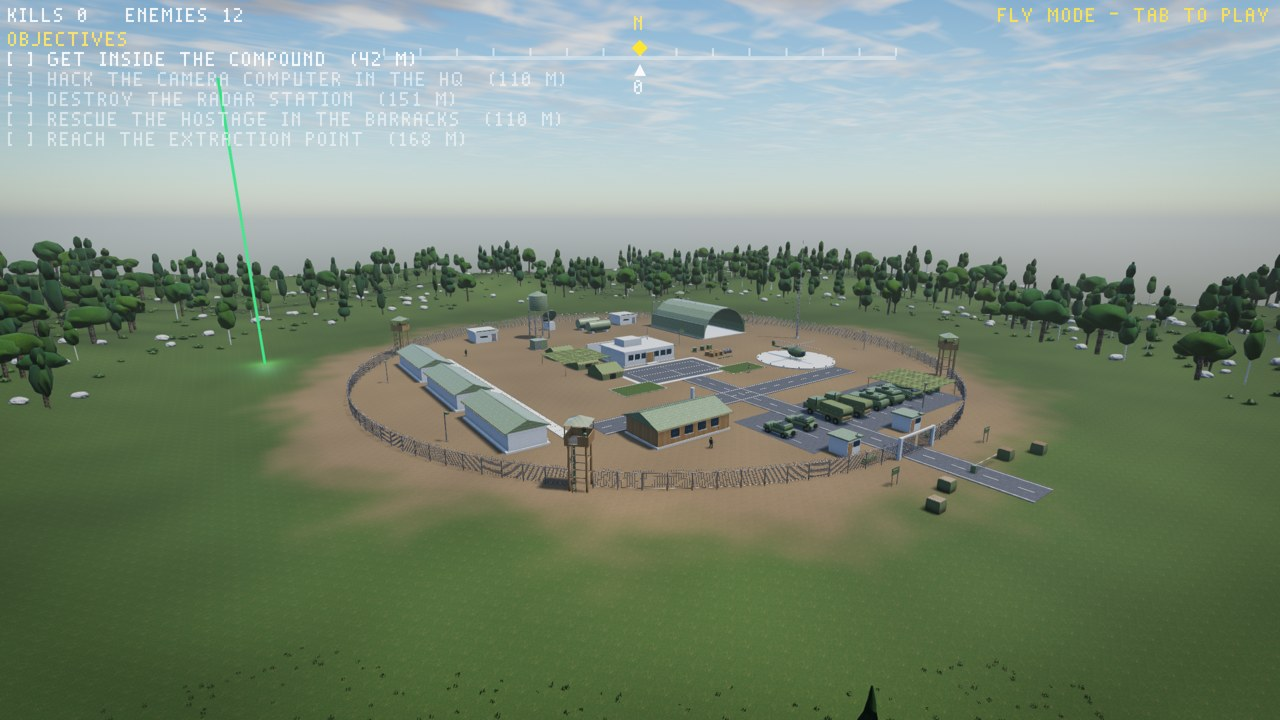
\includegraphics[width=\linewidth]{images/base.jpg}\caption{Base}\end{subfigure}\hfill
	\begin{subfigure}{0.31\linewidth}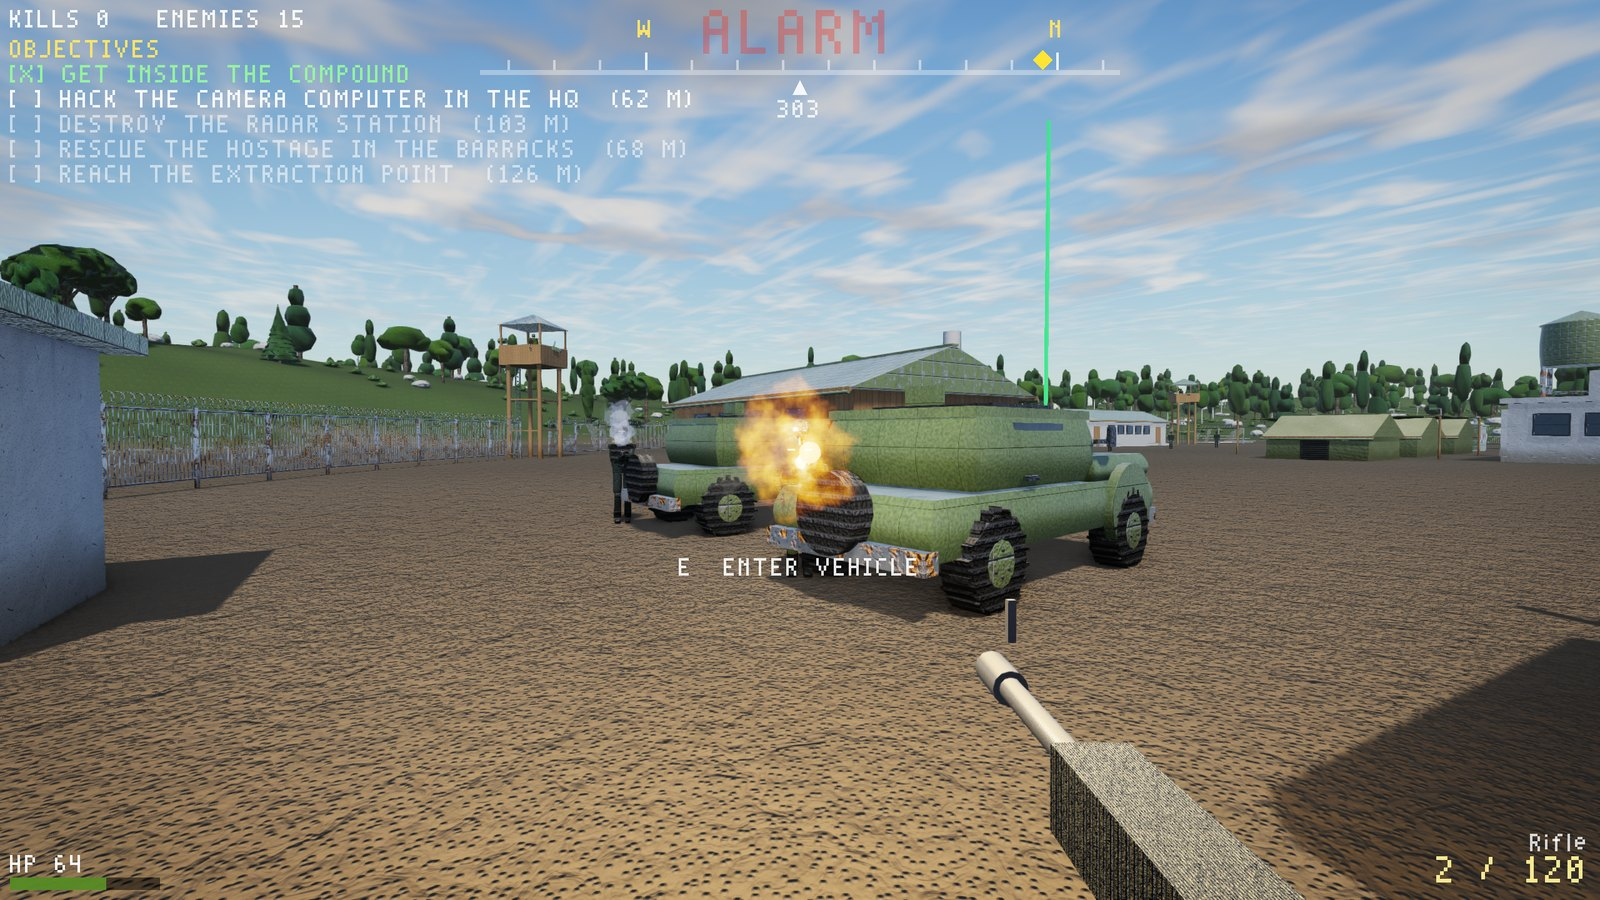
\includegraphics[width=\linewidth]{images/demo.jpg}\caption{Firefight}\end{subfigure}\hfill
	\begin{subfigure}{0.31\linewidth}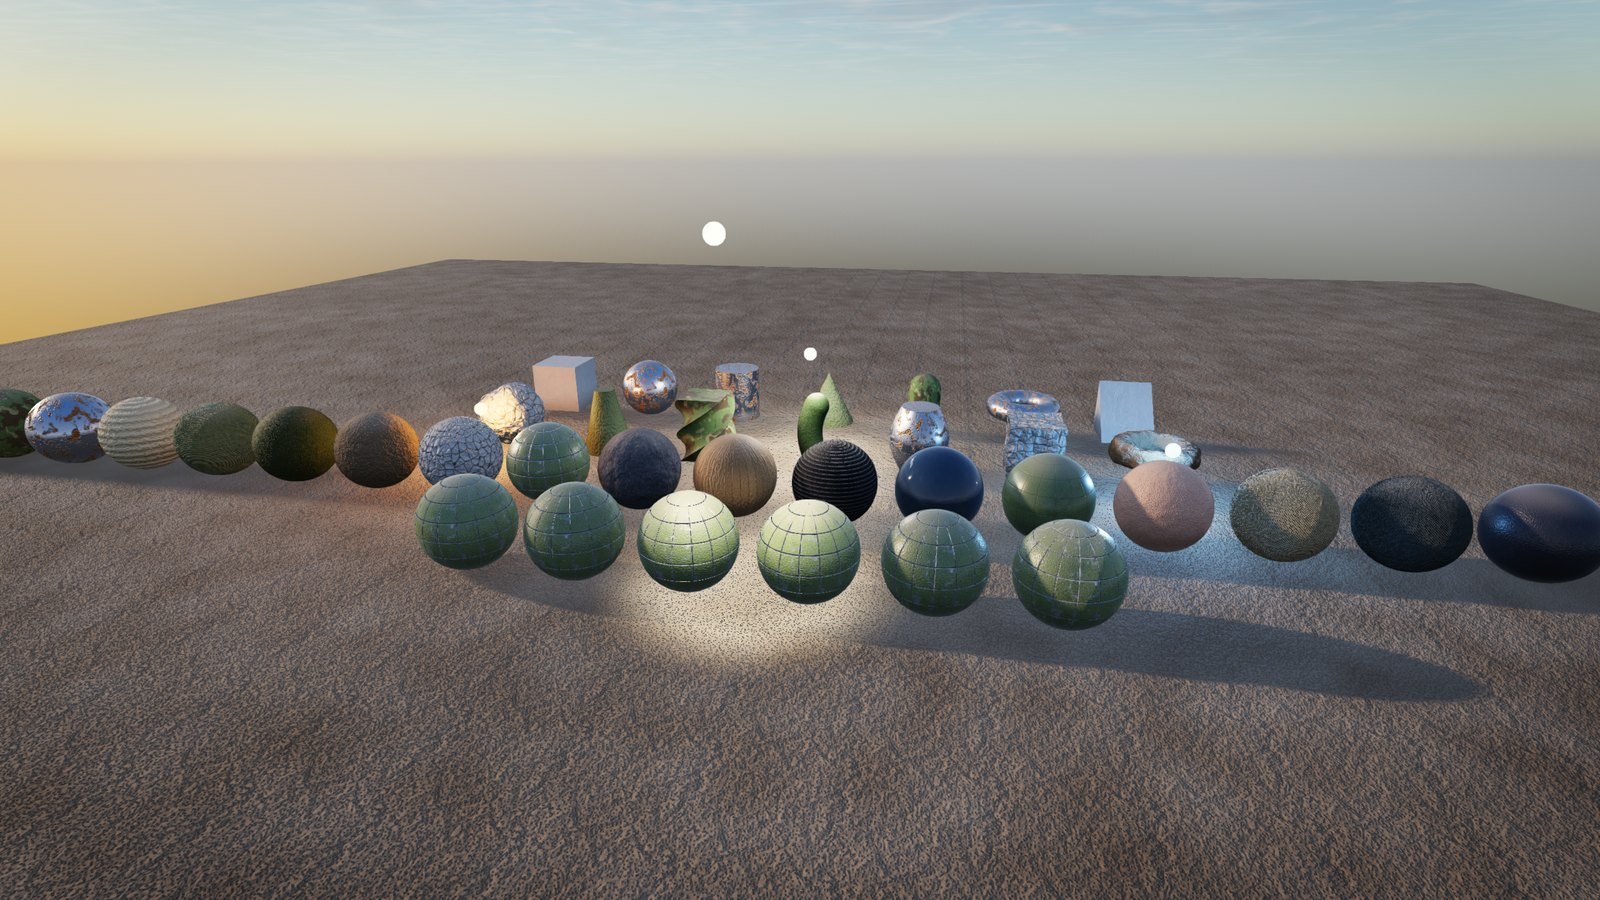
\includegraphics[width=\linewidth]{images/showroom.jpg}\caption{Materials}\end{subfigure}\\[2pt]
	\begin{subfigure}{0.31\linewidth}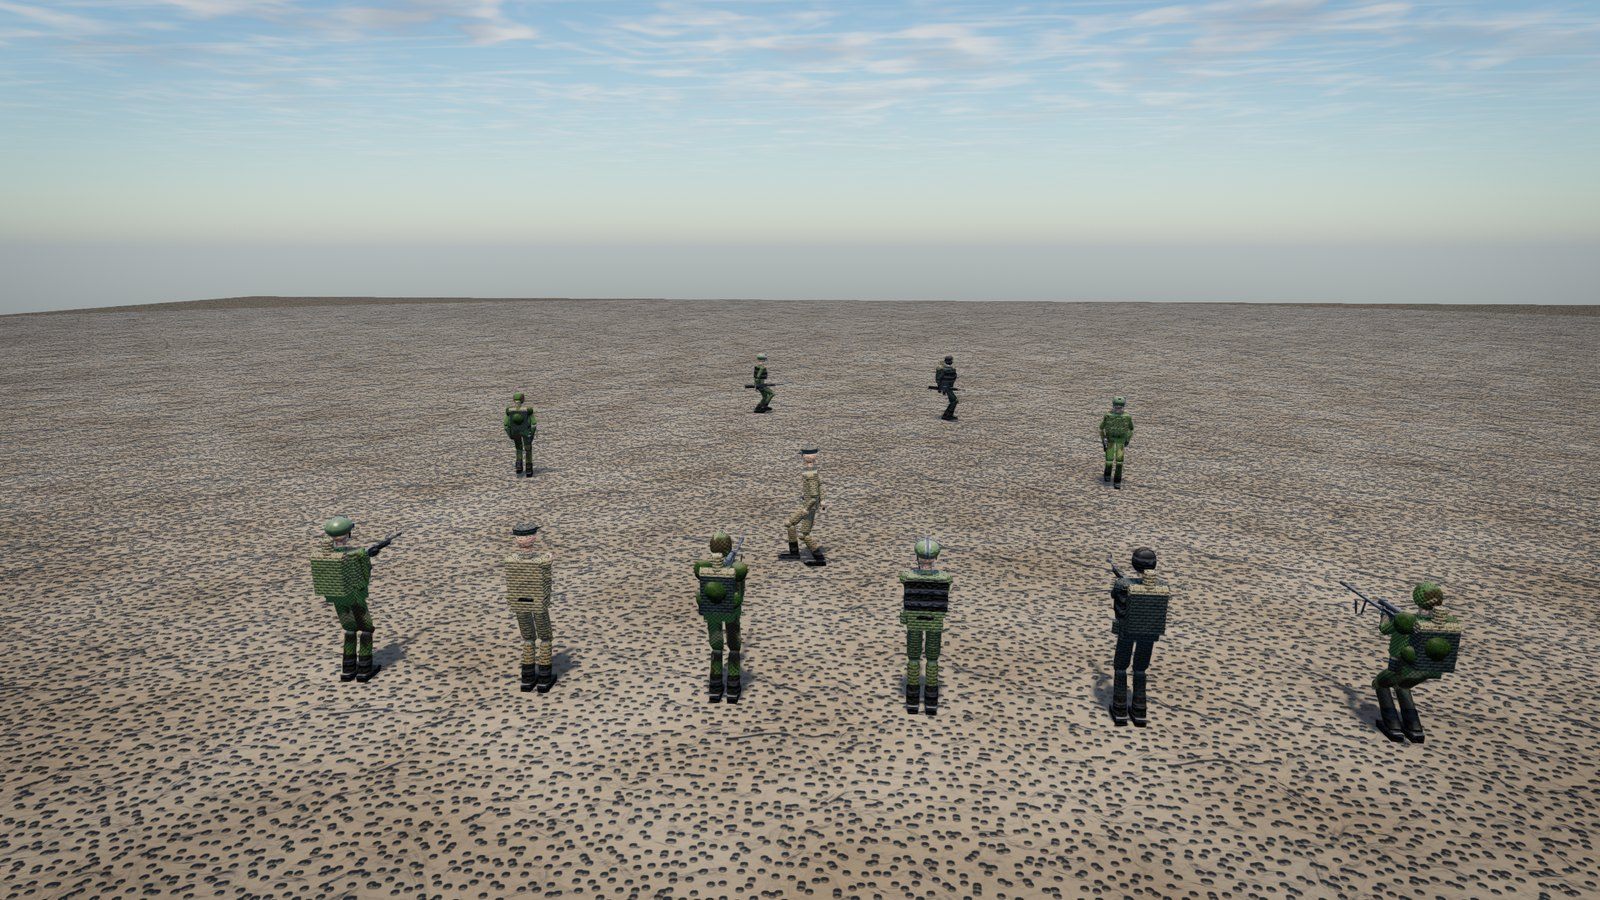
\includegraphics[width=\linewidth]{images/soldiers.jpg}\caption{Soldiers}\end{subfigure}\hfill
	\begin{subfigure}{0.31\linewidth}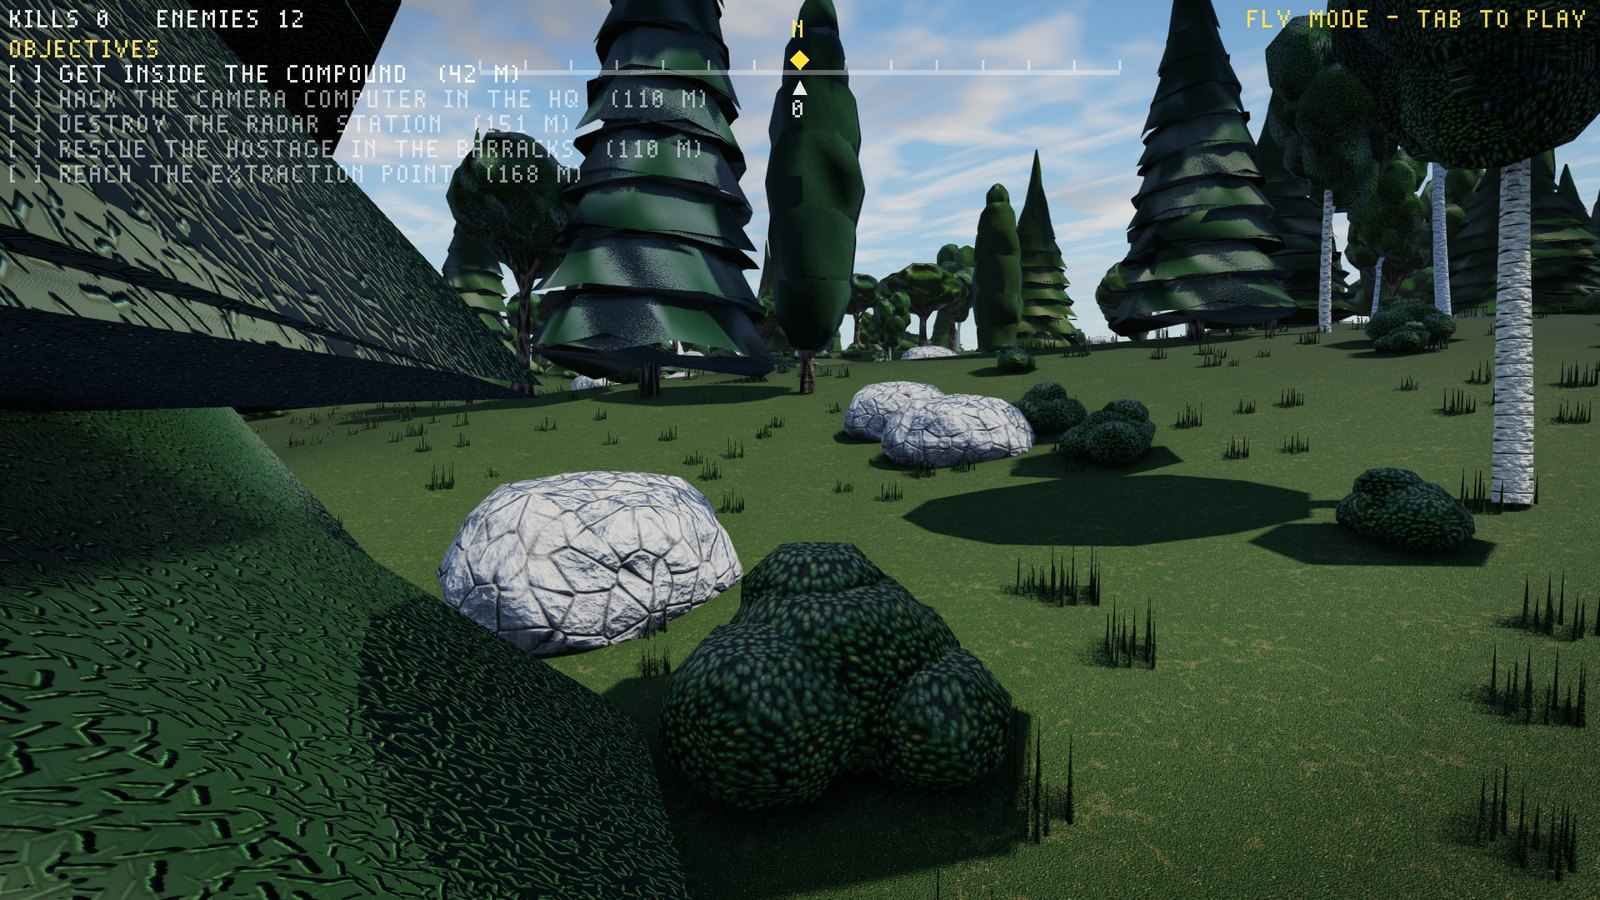
\includegraphics[width=\linewidth]{images/trees.jpg}\caption{Trees}\end{subfigure}\hfill
	\begin{subfigure}{0.31\linewidth}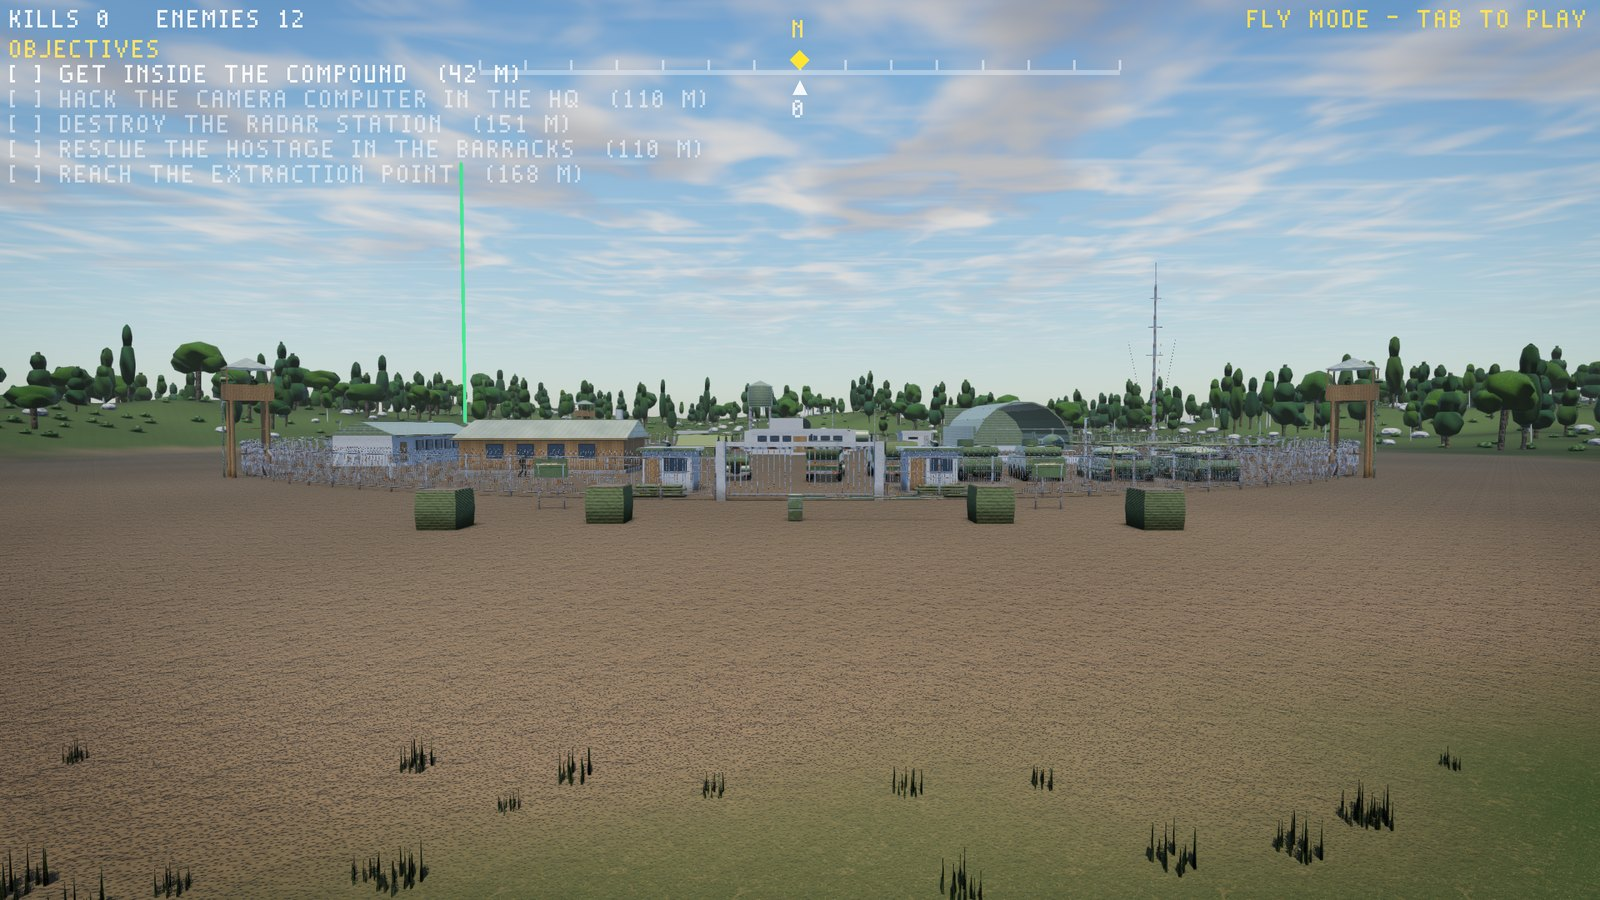
\includegraphics[width=\linewidth]{images/gate_day.jpg}\caption{Clouds}\end{subfigure}\\[2pt]
	\begin{subfigure}{0.31\linewidth}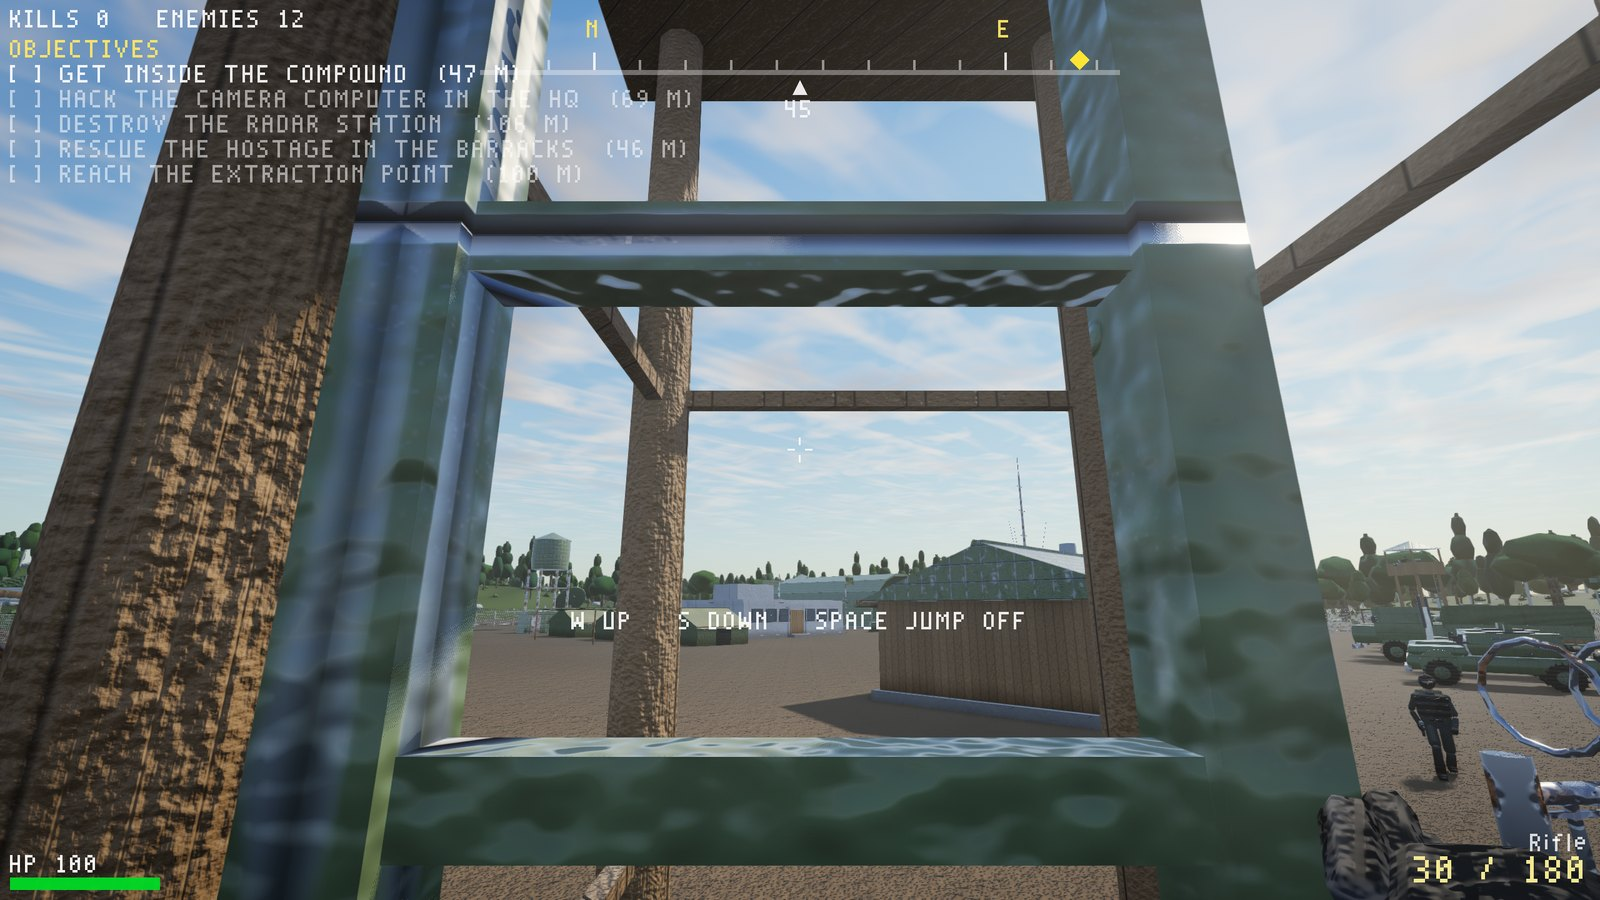
\includegraphics[width=\linewidth]{images/ladder.jpg}\caption{Ladder}\end{subfigure}\hfill
	\begin{subfigure}{0.31\linewidth}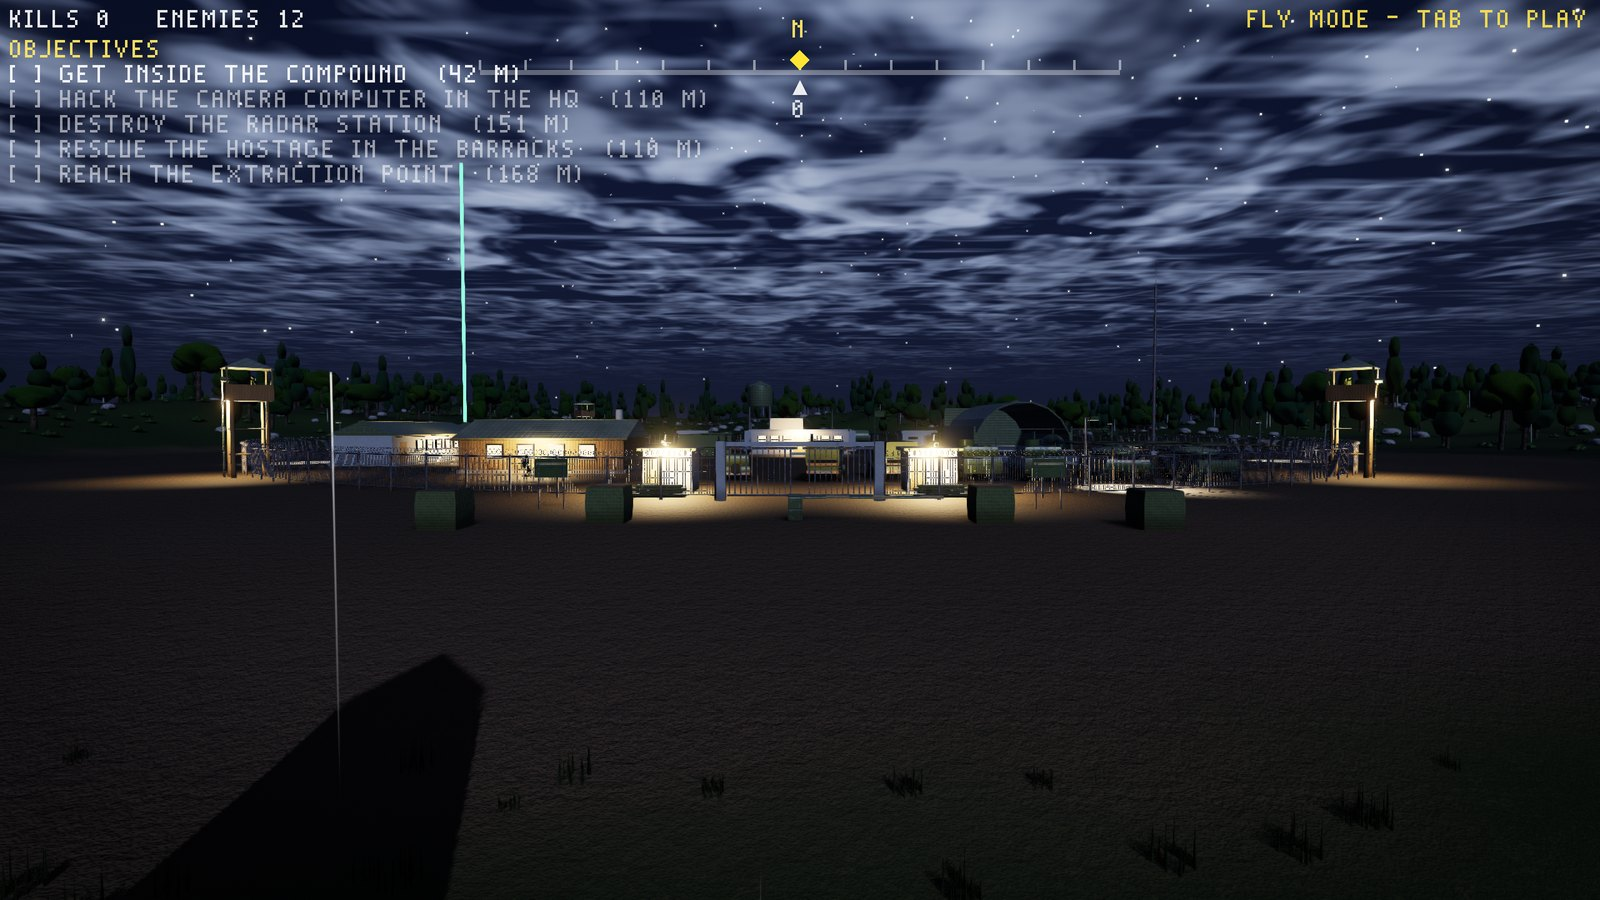
\includegraphics[width=\linewidth]{images/gate_night_bug.jpg}\caption{Night, bug}\end{subfigure}\hfill
	\begin{subfigure}{0.31\linewidth}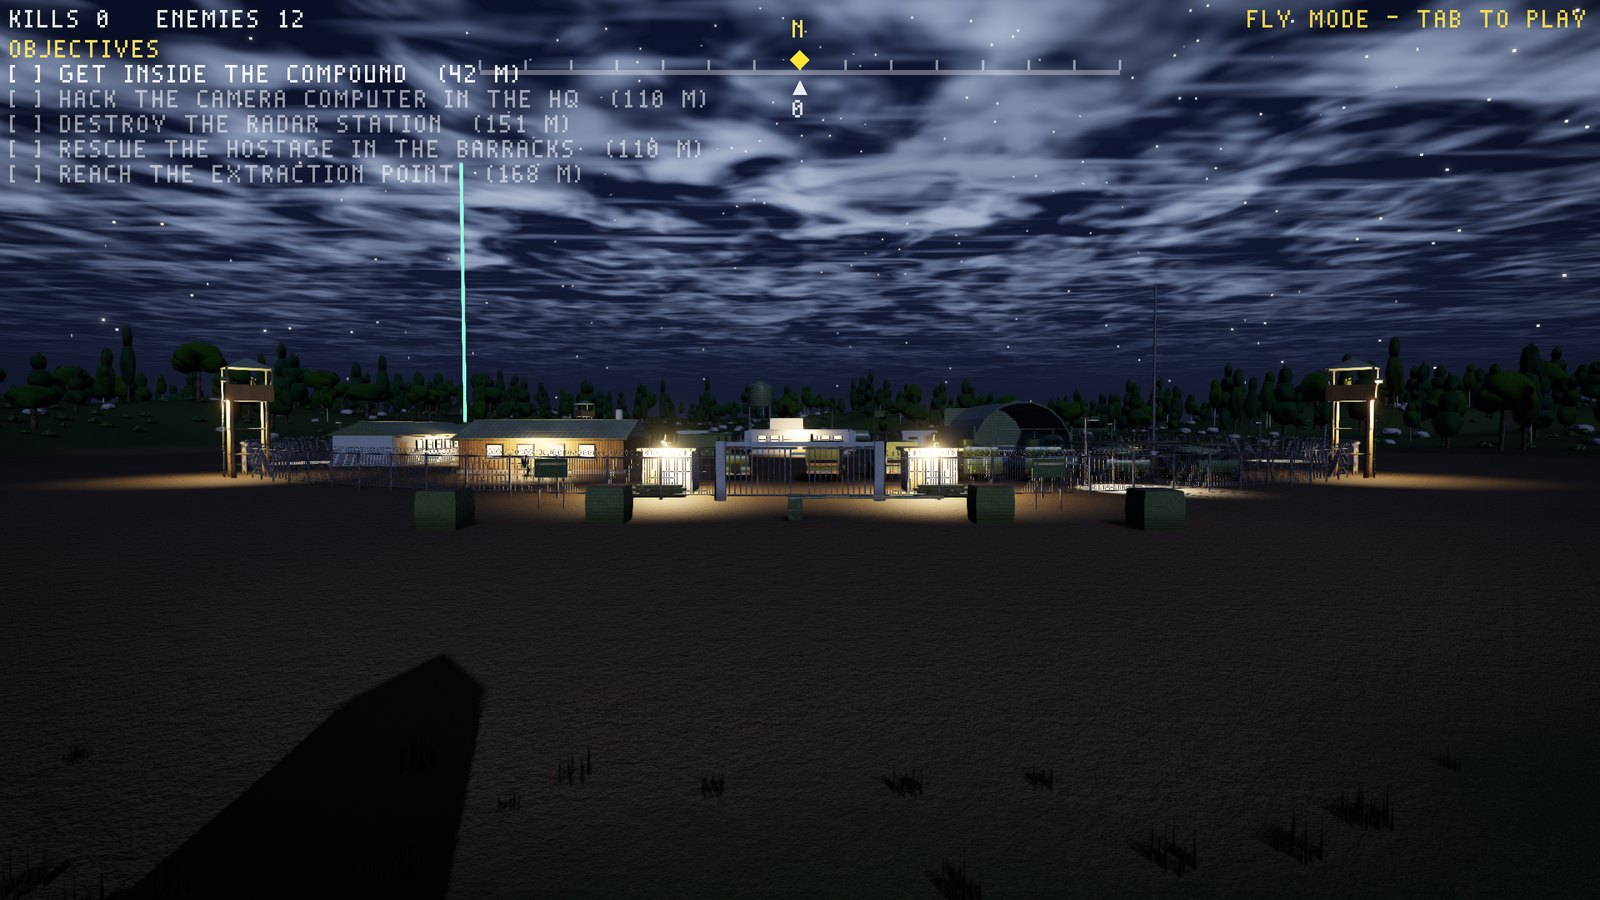
\includegraphics[width=\linewidth]{images/gate_night.jpg}\caption{Night, fixed}\end{subfigure}
	\caption{The engine and game in action; (h) and (i) show the streak bug and its fix.}\label{fig:shots1}
\end{figure}

\subsection{Analysis of the results}
Geometry costs most, so instancing and per-chunk culling matter. The streak was found by bisecting: removing draw items, lights and effects until it vanished.

\section{Objective Achieved}
(1) Six layers with downward-only dependencies. (2) No model, image or sound file: 22 materials, 4 tree species, 5 vehicles, synthesised audio. (3) Deferred PBR with shadows, SSAO, reflections, sky, clouds, bloom, ACES, FXAA. (4) Two playable missions with ladders, vehicles and stealth. (5) 281 tests, 327\,000 GL checks, 2 playthroughs, 10.9\,ms GPU time.

\section{Conclusion}
A procedural engine meets a 60 fps budget and passes exact checks.

% ============================================================
%  CHAPTER V
% ============================================================
\chapter{Societal, Health, Environment, Safety, Ethical, Legal and Cultural Issues}

\section{Intellectual Property Considerations}
All content is original; libraries are open source. The mission is inspired by, not copied from, \textit{Project I.G.I.}

\section{Ethical Considerations}
Fiction for adults; no personal data.

\section{Safety Considerations}
Short flashes, limited sound.

\section{Legal Considerations}
Licences respected; violence stylised; sources cited.

\section{Impact on Societal, Health and Cultural Issues}
Lowers the barrier to learning graphics; rescue and stealth goals temper shooting.

\section{Impact on the Environment and Sustainability}
No art downloads; display sync saves GPU work.

% ============================================================
%  CHAPTER VI
% ============================================================
\chapter{Addressing Complex Engineering Problems and Activities}

\section{Complex Engineering Problems}
\textbf{Depth of knowledge:} radiometry, noise, filters, GPU pipelines, state machines. \textbf{Conflicts:} realism versus a 16.7\,ms frame; no files versus rich surfaces; no compute shaders. \textbf{Analysis:} bisecting the star streak, proving tiling. \textbf{Interdependence:} renderer, world, game and audio share data and timing.

\section{Complex Engineering Activities}
The project used modern tools, integrated many components and verified quality by measurement.

% ============================================================
%  CHAPTER VII
% ============================================================
\chapter{Conclusions}

\section{Summary}
Sentinel shows that a complete 3D game, from surfaces and shapes to weather and sound, can be generated entirely by code under an OpenGL~4.1 limit: a six-layer engine, a deferred physically based renderer, noise-based recipes, table-driven objects and a mission game, in about 21\,000 lines within a 60 fps budget.

\section{Limitations}
Models are blocky; there is no true global illumination; foliage is lumpy volumes, not leaves; the beacon is a solid column; tuning used scripts and screenshots, not a large playtest.

\section{Recommendations and Future Works}
Leaf cards with cut-out transparency, screen-space global illumination, point-light shadows, multiplayer and a user study; a modern graphics API with compute shaders.

% ============================================================
%  REFERENCES
% ============================================================
\phantomsection
\addcontentsline{toc}{frontmatter}{References}
\vspace{6pt}
\begin{center}{\fontsize{14}{21}\bfseries\selectfont REFERENCES}\end{center}
\vspace{2pt}
\begin{spacing}{0.95}\scriptsize
\begin{enumerate}[leftmargin=0pt,itemindent=0pt,labelsep=0.5em,labelwidth=1.5em,itemsep=0pt,parsep=0pt,label={[\arabic*]},align=left]
	\item K.~Perlin, ``Improving noise,'' \textit{ACM Trans. Graph. (SIGGRAPH)}, vol.~21, no.~3, pp.~681--682, 2002.
	\item S.~Worley, ``A cellular texture basis function,'' in \textit{Proc. SIGGRAPH}, 1996, pp.~291--294.
	\item R.~L. Cook and K.~E. Torrance, ``A reflectance model for computer graphics,'' \textit{ACM Trans. Graph.}, vol.~1, no.~1, pp.~7--24, 1982.
	\item B.~Walter, S.~R. Marschner, H.~Li and K.~E. Torrance, ``Microfacet models for refraction through rough surfaces,'' in \textit{Proc. Eurographics Symp. Rendering}, 2007, pp.~195--206.
	\item B.~Karis, ``Real shading in Unreal Engine 4,'' SIGGRAPH Course: Physically Based Shading in Theory and Practice, 2013.
	\item S.~Hillaire, ``A scalable and production ready sky and atmosphere rendering technique,'' \textit{Computer Graphics Forum}, vol.~39, no.~4, pp.~13--22, 2020.
	\item R.~Dimitrov, ``Cascaded shadow maps,'' NVIDIA White Paper, 2007.
	\item M.~Oren and S.~K. Nayar, ``Generalization of Lambert's reflectance model,'' in \textit{Proc. SIGGRAPH}, 1994, pp.~239--246.
	\item K.~Narkowicz, ``ACES filmic tone mapping curve,'' blog post, 2016.
	\item J.~Jimenez, ``Next generation post processing in Call of Duty: Advanced Warfare,'' SIGGRAPH Course: Advances in Real-Time Rendering, 2014.
	\item T.~Lottes, ``FXAA,'' NVIDIA White Paper, 2009.
	\item M.~Segal and K.~Akeley, \textit{The OpenGL Graphics System: A Specification, Version 4.1}, Khronos Group, 2010.
	\item I.~Quilez, ``Domain warping,'' online article, iquilezles.org.
	\item S.~Hargreaves and M.~Harris, ``Deferred shading,'' NVIDIA presentation, Game Developers Conference, 2004.
	\item H.~Scharr, ``Optimal operators in digital image processing,'' Ph.D. dissertation, Univ. Heidelberg, 2000.
	\item T.~Akenine-M{\"o}ller, E.~Haines and N.~Hoffman, \textit{Real-Time Rendering}, 4th~ed., CRC Press, 2018.
\end{enumerate}
\end{spacing}

\end{document}
